\section{Importance of testing}
\setauthor{Romeo Bhuiyan}
Usability testing is a crucial evaluation method that is used to assess the user 
experience of a web application. It involves having real users perform tasks on a 
website or application and observing their interactions, behaviors, and feedback. 
The goal of usability testing is to determine if the web application is user-friendly, 
efficient, and intuitive for the target audience.

Usability testing is important for web applications for several reasons. First and 
foremost, it allows developers and designers to identify any usability issues before 
the application is released to the public. This can save significant time and money, 
as fixing these issues later in the development cycle can be more time-consuming and costly.

In addition, usability testing helps ensure that the application meets the needs 
and expectations of the target audience. This is essential in ensuring that the 
application is successful and meets the needs of its users. Usability testing 
can also help identify areas for improvement, such as navigation, page layout, 
and content organization.

Another benefit of usability testing is that it provides valuable insight 
into how users interact with the application. This can help developers 
and designers understand how users approach tasks and what their pain 
points are when using the application. This information can then be 
used to make improvements to the user experience and ensure that 
the application is as user-friendly as possible.
\\
\\
\section{Functional testing}
\setauthor{Romeo Bhuiyan}
\textbf{Functional testing} is a type of software testing that verifies the functionality of a system, application, or a component. 
The main objective of functional testing is to ensure that the system meets the specified requirements and works as expected. 
It is a comprehensive evaluation of the software's functionality, covering all possible scenarios and use cases. 
This type of testing focuses on evaluating the features, capabilities, and end-to-end behavior of the system.

That involves testing each individual function or feature of the system in isolation, and then 
integrating and testing the system as a whole. The testing process starts with the requirement analysis, 
where the system requirements are reviewed, understood and prioritized. Based on the requirements, 
the test cases are then designed and executed. During the testing process, the tester performs 
various tests such as unit testing, integration testing, system testing, and acceptance testing.

Functional testing is an essential step in the software development life cycle, as it helps to 
identify any defects or bugs in the system early in the development process. This helps to 
reduce the cost of fixing the defects and ensures that the software is delivered to the 
end-users with high quality and reliability.

That helps to validate the software's compliance with the business requirements 
and user expectations, thereby ensuring the software's overall quality and usability. 
It is important to perform functional testing on a regular basis to ensure that 
any new changes or updates made to the system do not affect its functionality and performance.


\section{Non-functional testing}
\setauthor{Romeo Bhuiyan}
\textbf{Non-functional testing} is a type of software testing that is performed to verify the non-functional aspects of a software system. 
It is concerned with evaluating the performance, reliability, usability, and security of a software system under different conditions. 
Non-functional testing is an important aspect of software development that helps ensure the overall quality of a software system.

This kind of testing can be categorized into several different types based on the specific aspect of the system being tested. 
Some of the common types of non-functional testing include performance testing, reliability testing, usability testing, 
security testing, compatibility testing, and scalability testing.

\textbf{Performance testing} is concerned with evaluating the performance of the software system under different conditions, 
such as high load or high traffic. This type of testing is usually performed to identify performance bottlenecks and 
to optimize the system for better performance.

\textbf{Reliability testing} is concerned with evaluating the reliability of the software system under different conditions, 
such as network failures or hardware failures. This type of testing is usually performed to identify potential failures 
in the system and to ensure that the system is reliable under all possible conditions.

\texttt{Usability testing} is concerned with evaluating the usability of the software system from the user's perspective. This 
type of testing is usually performed to ensure that the system is easy to use and that it meets the user's expectations.

\textbf{Security testing} is concerned with evaluating the security of the software system from different types of threats, such as 
hacking or virus attacks. This type of testing is usually performed to identify potential security vulnerabilities in the 
system and to ensure that the system is secure under all possible conditions.

\textbf{Compatibility testing} is concerned with evaluating the compatibility of the software system with different types of hardware 
and software configurations. This type of testing is usually performed to ensure that the system works correctly on different 
types of devices and with different types of software configurations.

\textbf{Scalability testing} is concerned with evaluating the scalability of the software system under different conditions, such as 
increased user traffic or increased data volume. This type of testing is usually performed to identify potential scalability 
issues in the system and to ensure that the system can handle increased load without any performance degradation.

\section{Focus Groups}
\setauthor{Romeo Bhuiyan}
Face and body tracking technology has rapidly advanced in recent years, providing significant benefits to various industries, 
including gaming, healthcare, security, and entertainment. The technology enables the tracking of facial expressions, body movements, 
and gestures, allowing for a more immersive and interactive experience. In this text, we will focus on the focus group of face and body 
tracking technology, its advantages, and several examples of its application.

A focus group is a research methodology that aims to gather data from a group of individuals about their attitudes, opinions, 
and behaviors concerning a particular topic. In the case of face and body tracking technology, a focus group could consist of 
individuals who have used or are interested in using the technology. The focus group would provide insights into the experiences, 
opinions, and potential applications of the technology, which could be beneficial to developers and manufacturers.

One advantage of face and body tracking technology is its potential for use in healthcare. The technology can be used to track 
the movement and progress of patients during rehabilitation, allowing doctors and therapists to monitor their progress 
and adjust treatment plans accordingly. For example, a patient recovering from a stroke could use a device equipped 
with face and body tracking technology to monitor their movements and receive feedback on their progress. 
The technology can also be used to detect early signs of conditions such as Parkinson's disease, allowing for early intervention and treatment.

Another potential application of face and body tracking technology is in the gaming industry. 
The technology can be used to create more immersive and interactive gaming experiences, allowing 
players to control characters with their movements and facial expressions. For example, the game 
"Just Dance" uses face and body tracking technology to detect the player's movements and provide 
feedback on their performance. Similarly, the game "The Climb" uses the technology to simulate rock 
climbing, allowing players to control their character's movements with their own.

In the field of security, face and body tracking technology can be used to enhance surveillance systems, making them 
more accurate and effective. The technology can be used to track individuals as they move through a space, providing real-time 
information on their location and movements. This information can be used to identify potential threats and respond quickly 
to incidents. For example, a security system equipped with face and body tracking technology could detect a suspicious 
individual entering a restricted area and alert security personnel to take action.

The entertainment industry has also embraced face and body tracking technology, using it to create more engaging and 
interactive experiences for audiences. The technology can be used to track the movements and expressions of performers, 
allowing them to control animated characters or special effects in real-time. For example, the Cirque du Soleil show "KÀ" uses face and body 
tracking technology to create a seamless blend of live performance and digital effects, enhancing the audience's experience. \cite{cirque}

\subsection{Virtual Youtubers as a trend}
\setauthor{Romeo Bhuiyan}
VTubing, or virtual YouTubing, is a rapidly growing trend that utilizes face and body tracking 
technology to create animated characters that interact with audiences in real-time. The technology allows users to 
create virtual personas that can be controlled using their own facial expressions and movements. 
This has led to the development of a vibrant community of VTubers, who create content and interact with their 
audiences through their virtual personas.

The community of VTubers has grown significantly in recent years, with many creators gaining massive followings 
and attracting a global audience. The use of face and body tracking technology allows these creators to create 
unique and engaging content, with their virtual personas often taking on a life of their own. The technology 
also provides opportunities for creative expression, with VTubers able to experiment with different character 
designs and personality traits.

The community of VTubers has also given rise to new forms of entertainment and social interaction. Virtual 
concerts and live streams have become increasingly popular, with VTubers able to engage with their audiences 
in real-time and create personalized experiences. The community has also developed its own set of memes, 
catchphrases, and cultural references, contributing to the unique identity of VTubing as a cultural phenomenon.
\\
\begin{figure}[htb]
    \centering
    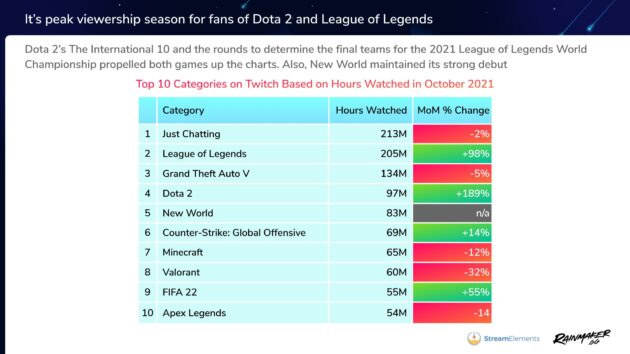
\includegraphics[width=0.9\textwidth]{pics/justchattwitch.jpg}
    \caption{Popularity of different Twitch categories 2021}
    \cite{geekwire}
    \label{fig:justchattwitch}
\end{figure}
\\
Twitch's \emph{Just Chatting} category has been rapidly growing in popularity since its inception in 2018. The category allows streamers 
to interact with their audience in a more casual and personal setting, providing a space for non-gaming related content such as chatting, 
storytelling, and socializing. The category has become one of the most popular on Twitch, with thousands of streamers and millions of 
viewers tuning in every day, as shown in the figure \ref{fig:justchattwitch} above.

One of the reasons for the popularity of \emph{Just Chatting} on Twitch is the increasing trend of content creators who are more 
personality-driven than gameplay-driven. These streamers use their charisma, humor, and relatability to attract viewers and build 
communities. They often share personal stories and insights, provide advice, or just hang out and chat with their audience. 
The conversational format of \emph{Just Chatting} allows these streamers to create a more intimate connection with their fans, 
leading to increased engagement and loyalty.

Another reason for the popularity of \emph{Just Chatting} is the rise of Virtual YouTubers, or VTubers. VTubers are 
digital avatars controlled by real people, who interact with their audience through live streams and pre-recorded videos. 
The trend originated in Japan but has since spread worldwide, with many VTubers gaining millions of followers on various 
platforms, including Twitch. VTubers have added a new dimension to the \emph{Just Chatting} category, as they provide a unique 
and entertaining way of connecting with fans. VTubers can also interact with other streamers, creating a dynamic and collaborative community.

The appeal of VTubers lies in their ability to create a fictional character that embodies their personality and traits. 
Fans can easily connect with these avatars, as they often represent a version of the streamer's ideal self. The anonymity 
provided by the digital avatar allows VTubers to be more open and expressive, which adds to the entertainment value of their 
streams. VTubers also bring a level of creativity to the \emph{Just Chatting} category, as they often use animations, sound effects, 
and other visual elements to enhance their streams.

\section{Materiality of CrowdFit}
\setauthor{Romeo Bhuiyan}
CrowdFit is a powerful tool that can help new products succeed in the market. It's a method of gathering feedback and insights from a 
large group of people, often through social media, online forums, or other digital platforms. This approach allows businesses 
to tap into the collective knowledge and experiences of their target audience, providing valuable insights into customer needs and preferences.

One of the biggest advantages of using CrowdFit is that it can provide businesses with a more accurate understanding of their 
target market. By gathering feedback from a diverse range of individuals, businesses can gain insights into the needs and desires 
of their target audience that they may not have otherwise discovered. This can help businesses develop products that are more 
tailored to the needs of their customers, ultimately leading to increased sales and customer satisfaction.

Another advantage of CrowdFit is that it can help businesses identify potential issues or problems with their product before it 
is launched. By gathering feedback from a large group of people, businesses can identify any potential issues or areas for improvement, 
allowing them to make changes to the product before it is released. This can save businesses time and money in the long run, as it can 
prevent the need for costly recalls or other remedial actions.

CrowdFit can also help businesses build brand awareness and loyalty. By engaging with their target audience and demonstrating that they 
value their opinions, businesses can foster a sense of community and connection with their customers. This can lead to increased brand 
loyalty and positive word-of-mouth marketing, both of which are crucial for the success of any new product.

One of the key benefits of CrowdFit is that it is a relatively low-cost method of gathering feedback and insights from customers. 
Traditional market research methods, such as focus groups or surveys, can be expensive and time-consuming. CrowdFit, on the other hand, 
can be done quickly and easily using social media or other digital platforms, making it a more accessible option for businesses with limited resources.

\section{Run session}
\setauthor{Romeo Bhuiyan}
Run sessions are an integral part of usability testing, and they play a crucial role in ensuring the success of the testing process. 
A run session refers to a single instance of a usability testing activity, where participants are observed while performing various 
tasks on a product or system. These sessions are conducted by usability experts who collect and analyze data to identify user behavior 
and to identify any design or usability issues.
The importance of run sessions in usability testing cannot be overstated. They provide valuable insights into how users interact with a 
product or system, and they help designers and developers make informed decisions about how to improve the product's usability. 
There are several reasons why run sessions are so important, including the following below.

\subsection{Identify usability issues}
\setauthor{Romeo Bhuiyan}
The primary goal of usability testing is to identify usability issues and improve the product's overall usability. 
Run sessions help designers and developers identify these issues by providing real-world feedback on how users interact 
with the product. This feedback can include issues with navigation, layout, content, or functionality, among other things.

\subsection{Obtain user feedback}
\setauthor{Romeo Bhuiyan}
Run sessions also provide an opportunity to obtain direct feedback from users. By observing how users interact 
with the product, usability experts can ask questions and gather feedback on what users like, dislike, or find 
confusing about the product. This feedback can be used to inform design decisions and make improvements to the product.

\subsection{Test assumptions}
\setauthor{Romeo Bhuiyan}
Designers and developers often make assumptions about how users will interact with a product. Run sessions 
provide an opportunity to test these assumptions and validate or challenge them. This is particularly important 
because assumptions that go untested can lead to costly design errors and usability issues.

\subsection{Improve product quality}
\setauthor{Romeo Bhuiyan}
Usability testing, and run sessions in particular, can significantly improve the quality of a product. 
By identifying usability issues and obtaining user feedback, designers and developers can make informed 
decisions about how to improve the product's usability. This can lead to a better user experience, 
increased user satisfaction, and ultimately, better product adoption.

\subsection{Increase efficiency}
\setauthor{Romeo Bhuiyan}
Finally, run sessions can also increase the efficiency of the design and development process. 
By identifying usability issues early in the process, designers and developers can make changes 
before the product is released, saving time and resources. Additionally, usability testing can 
help to prevent costly design errors and product recalls.

\section{Use cases}
\setauthor{Romeo Bhuiyan}
Face and body tracking software is a type of technology that is designed to track and analyze the movements and positions 
of a person's face and body in real-time. This technology has many potential use cases across a wide range of industries, 
from marketing and advertising to gaming and entertainment.

One use case for face and body tracking software is in the retail industry. Retailers can use this technology to track 
where customers are looking and what products they are interested in. By analyzing customer behavior and preferences, 
retailers can optimize their product placement and marketing strategies to increase sales and improve customer engagement. 
For example, a supermarket could use face and body tracking software to determine which products are most popular, where 
customers tend to linger, and which areas of the store are most frequently visited.

Another potential use case for face and body tracking software is in the field of virtual reality and gaming. This 
technology can be used to create more immersive and interactive gaming experiences by tracking the player's movements 
and actions in real-time. For example, a game developer could use this technology to create a virtual reality game 
where the player's movements are tracked and translated into in-game actions, allowing for a more realistic and 
engaging experience.

In the world of entertainment, face and body tracking software is becoming increasingly popular for creating virtual 
avatars, also known as Vtubing. This technology allows content creators to create digital avatars that mimic their 
facial expressions and body movements in real-time, making it possible to create live streams and videos with a 
virtual character as the main presenter. This has opened up new possibilities for content creation and entertainment, 
with Vtubers becoming increasingly popular on platforms like Twitch and YouTube.

In the healthcare industry, face and body tracking software can be used to help diagnose and treat medical conditions. 
For example, it could be used to track the movements of patients with Parkinson's disease, allowing doctors to monitor 
their symptoms and adjust their treatment plans accordingly.

In the field of education, face and body tracking software can be used to track student engagement and improve teaching 
techniques. For example, it could be used to monitor student eye movements and facial expressions during lectures, allowing 
teachers to adjust their teaching style and content to better engage their students.

\section{Test Report}
\setauthor{Romeo Bhuiyan}
The purpose of this report is to provide a comprehensive analysis of the usability testing of Animotion, a web application that uses face and 
body tracking technology. The usability testing was conducted with a total of 116 participants who were categorized by age and experience 
with information technology and artificial intelligence. The report will discuss the results of the testing and provide recommendations for future improvements.

\subsection{Methodology}
\setauthor{Romeo Bhuiyan}
The usability testing was conducted with a total of 116 participants, consisting of 84 people aged between 12 and 15 years old with little experience 
with information technology and artificial intelligence, three people over 30 years old with some experience in these areas, and 29 people 
between 16 and 30 years old with high experience. Participants were selected from the Tadeot of the HTL Leonding in Austria. 
The testing was conducted in a controlled environment with participants seated in front of a computer screen.

Participants were given a brief explanation of what Animotion does and were then asked to use the web application to track 
their face and body movements. They were also asked to provide feedback on the application's ease of use, the accuracy of the tracking, and any issues 
they encountered while using the application.

\subsection{Result}
\setauthor{Romeo Bhuiyan}
The results of the usability testing were generally positive. Of the self-evaluated data, 95.14 \% of participants were able to intuitively 
understand what the application did without needing an explanation. This indicates that Animotion is user-friendly and easy to understand for most users.

However, the testing revealed that there were some issues with the application's accuracy in tracking face and body 
movements. Some participants reported that the tracking was not as precise as they expected, and that it was difficult to get the 
application to respond to their movements.

In addition, some participants noted that the application was not as intuitive to use as they expected. This was particularly true for the younger 
ones, who had less experience with information technology and artificial intelligence. They reported that the application was not always easy to navigate, 
and that they had difficulty understanding some of the features.

\subsection{Conclusion}
\setauthor{Romoe Bhuiyan}
In conclusion, the usability testing of Animotion showed that the web application is generally effective and user-friendly. 
However, there were some issues with the accuracy of the tracking technology and the application's ease of use. 
By prioritizing these areas and consistently seeking feedback from users, enhancements can be made to the application 
that will increase its usability and efficacy.